\documentclass[11pt,reqno]{amsart}
\usepackage{epsfig}
\usepackage{graphicx}
\usepackage{booktabs}
\usepackage{amsfonts}
\usepackage{amsmath}
\usepackage{amssymb}
%\usepackage{mathrsfs}
\usepackage[dvips=true]{hyperref}
\setcounter{MaxMatrixCols}{10}
\hfuzz=12pt
\hbadness=5000
\vbadness=5000
\frenchspacing
\vfuzz=2pt
\input{epsf}
%\input{tcilatex}

\begin{document}

\title[Bootstrapping the Illiquidity]{Bootstrapping the Illiquidity \\
\vspace{0.2cm}
\footnotesize{\emph{Multiple Yield Curves Construction \\
                    For Market Coherent Forward Rates Estimation}}}

\author{Ferdinando M. Ametrano}
\address{Financial Engineering, Banca IMI, Piazzetta G. Dell'Amore 3, 20121
Milan Italy, ferdinando.ametrano(AT)bancaimi.com}

\author{Marco Bianchetti}
\address{Risk Management, Banca IntesaSanpaolo, Piazza G. Ferrari 10, 20121
Milan Italy, marco.bianchetti(AT)intesasanpaolo.com}

\thanks{JEL Classifications: E45, G13. \\
The authors acknowledge fruitful discussions with S. De Nuccio, R. Giura, C. Maffi, F. Mercurio, N. Moreni, S. Pichugov and the QuantLib community. The opinions expressed here are solely of the authors and do not represent in any way those of theirs employers.}

\date{March 10th, 2009}

\keywords{liquidity crisis, credit crunch, interest rates, yield curve, forward curve, discount curve, bootstrapping, pricing, hedging, interest rate derivatives, Deposit, FRA, Futures, Swap, Basis Swap, turn of year, spline, QuantLib.}

\begin{abstract}
The large basis spreads observed on the interest rate market since the liquidity crisis of summer 2007 imply that different yield curves are required for market coherent estimation of forward rates with different tenors (e.g. Euribor 3 months, Euribor 6 months, etc.).
\par
In this paper we review the methodology for bootstrapping multiple interest rate yield curves, each homogeneous in the underlying rate tenor, from non-homogeneous plain vanilla instruments quoted on the market, such as Deposits, Forward Rate Agreements, Futures, Swaps, and Basis Swaps.
The approach includes turn of year effects and is robust to deliver smooth yield curves and to ensure non-negative rates also in highly stressed market situations, characterized by crazy roller coaster shapes of the market quotations.
\par
The concrete EUR market case is analyzed in detail, using the open source QuantLib implementation of the proposed algorithms.
\end{abstract}

\maketitle
%\tableofcontents

\section{Introduction}
\label{sec:Intro}
Pricing complex interest rate derivatives requires modeling the future dynamics of the yield curve term structure. Most of the literature assumes the existence of the \emph{current} yield curve as given, and its construction is often neglected, or even obscured, as it is considered more an art than a science. Actually any yield curve term structure modeling approach will fail to produce good/reasonable prices if the current term structure is not correct.
\par
Financial institutions, software houses and practitioners have developed their own proprietary methodologies in order to extract the yield curve term structure from quoted prices of a finite number of liquid market instruments.
\textquotedblleft Best-fit\textquotedblright\ algorithms assume a smooth functional form for the term structure and calibrate its parameters such that to minimize the repricing error of the chosen set of calibration instruments. For instance, the European Central Bank publishes yield curves on the basis of the Soderlind and Svensson model \cite{SodSwe1997}, which is an extension of the Nelson-Siegel model (see e.g. refs. \cite{NelSie1987}, \cite{ChrDie07} and \cite{Cor08}). Such approach is popular due to the smoothness of the curve, calibration easiness, intuitive financial interpretation of functional form parameters (level, slope, curvature) and correspondence with principal component analysis. On the other side, the fit quality is typically not good enough for trading purposes in liquid markets.
\par
In practice \textquotedblleft exact-fit\textquotedblright\ algorithms are often preferred: they fix the yield curve on a time grid of $N$ points (pillars) in order to \emph{exactly} reprice $N$ pre-selected market instruments. The implementation of such algorithms is often incremental, extending the yield curve step-by-step with the increasing maturity of the ordered instruments, in a so called \textquotedblleft bootstrap\textquotedblright approach. Intermediate yield curve values are obtained by interpolation on the bootstrapping grid. Here different interpolation algorithms are available but little attention has been devoted in the literature to the fact that interpolation is often already used during bootstrapping, not just after that, and that the interaction between bootstrapping and interpolation can be subtle if not nasty (see e.g. \cite{HagWes06}, \cite{HagWes08}).
\par
Whilst naive algorithms may fail to deal with market subtleties such as date conventions, the intra-day fixing of the first floating payment of a Swap, the turn-of-year effect, the Futures convexity adjustment, etc., even very sophisticated algorithms used in a naive way may fail to estimate correct forward Euribor rates in difficult market conditions, as those observed since the summer of 2007 in occasion of the so-called {\it subprime credit crunch crisis.}
Namely using just one single curve is not enough to account for forward rates of different tenor, such as 1, 3, 6, 12 months, because of the large Basis Swap spreads presently quoted on the market.
\par
The plan of the paper is as follows:
in section \ref{sec:Pricing} we start by reviewing the traditional (old style) single curve market practice for pricing and hedging interest rate derivatives and the recent market evolution, triggered by the credit crunch crisis, towards a double-curve approach.
In section \ref{sec:Math} we fix the notation and nomenclature.
In section \ref{sec:SingleBootstrapping} we briefly summarize the traditional pre-credit crunch yield curve construction methodology.

In section \ref{sec:MultiBootstrapping}, that constitutes the central contribution of this work, we describe in great detail the new post-credit crunch multi-curve approach; in particular in its nine subsections we discuss the general features of the bootstrapping procedure, we review in detail the (EUR) market instruments available for yield curves construction, and we deal with some issues crucial for bootstrapping, in particular the fundamental role played by the interpolation scheme adopted (sec. \ref{sec:Interp}) and the incorporation of the turn-of-year effect (\ref{sec:TOY}).
Finally, in section \ref{sec:ImplementResults} we show an example of numerical results for the Euribor1M, 3M, 6M and 12M forward curves bootstrapping using the open source implementation released within the QuantLib framework.
The conclusions are collected in section \ref{sec:Conclusions}.

\section{Pre and Post Credit Crunch Pricing \& Hedging Interest Rate Derivatives}
\label{sec:Pricing}
One of the many consequences of the credit and liquidity crisis started in the second half of 2007 has been a strong increase of the basis spreads quoted on the market between single-currency interest rate instruments, Swaps in particular, characterized by different underlying rate tenors (e.g. Euribor3M\footnote{Euro Interbank Offered Rate, the rate at which euro interbank term Deposits within the euro zone are offered by one prime bank to another prime bank (see e.g. www.euribor.org).}, Euribor6M, etc.), reflecting the increased liquidity risk and the corresponding preference of financial institutions for receiving payments with higher frequency (quarterly instead of semi-annually, for instance).
\par
There are also other indicators of regime changes in the interest rate markets, such as the divergence between Deposit (Euribor based) and OIS (Overnight Indexed Swaps, Eonia\footnote{Euro OverNight Index Average, the rate computed as a weighted average of all overnight rates corresponding to unsecured lending transactions in the euro-zone interbank market (see e.g. \url{http://www.euribor.org}).} based) rates with the same maturity, or between FRA (Forward Rate Agreement) contacts and the corresponding forward rates implied by consecutive Deposits.
We stress that such situation is not completely new on the market: non-zero basis swap spreads were already quoted and understood before the crisis (see e.g. ref. \cite{TucPor03}), but their magnitude was very small and traditionally neglected (see also the discussion in refs. \cite{Mor08}, \cite{Mer09}).
\par
The asymmetries cited above have also induced a sort of "segmentation" of the interest rate market into sub-areas, mainly corresponding to instruments with 1M, 3M, 6M, 12M underlying rate tenors, characterized, in principle, by different internal dynamics, liquidity and credit risk premia, reflecting the different views and interests of the market players.
\par
The evolution of the financial markets briefly described above has triggered a general reflection about the methodology used to price and hedge interest rate derivatives, namely those financial instruments whose price depends on the present value of future interest rate-linked cashflows, that we review in the next two sections.

\subsection{\label{sec:SingleCurve}The Traditional Single Curve Approach}
\par
The pre-crisis standard market practice can be summarized in the following procedure (see e.g. refs. \cite{Ron00}, \cite{HagWes06}, \cite{And07} \cite{HagWes08}):
\begin{enumerate}
\item select \emph{one} finite set of the most convenient (e.g. liquid) vanilla interest rate instruments traded in real time on the market with increasing maturities; for instance, a very common choice in the EUR market is a combination of short-term EUR Deposit, medium-term Futures on Euribor3M and medium-long-term Swaps on Euribor6M;

\item build \emph{one} yield curve using the selected instruments plus a set of bootstrapping rules (e.g. pillars, priorities, interpolation, etc.);

\item compute \emph{on the same curve} forward rates, cashflows\footnote{within the present context of interest rate derivatives we focus in particular on forward rate dependent cashflows.}, discount factors and work out the prices by summing up the discounted cashflows;

\item compute the delta sensitivity and hedge the resulting delta risk using the suggested amounts (hedge ratios) of the \emph{same} set of vanillas.
\end{enumerate}
For instance, a 5.5Y maturity EUR floating Swap leg on Euribor1M (not directly quoted on the market) is commonly priced using discount factors and forward rates calculated on the same Depo-Futures-Swap curve cited above. The corresponding delta sensitivity is calculated by shocking one by one the curve pillars and the resulting delta risk is hedged using the suggested amounts (hedge ratios)\ of 5Y and 6Y Euribor6M Swaps\footnote{we refer here to the case of local yield curve bootstrapping methods, for which there are no sensitivity delocalization effect (see refs. \cite{HagWes06}, \cite{And07} \cite{HagWes08}).}.
\par
We stress that this is a \emph{single-currency-single-curve approach}, in that a \emph{unique} curve is built and used to price and hedge any interest rate derivative on a given currency. Thinking in terms of more fundamental variables, e.g. the short rate, this is equivalent to assume that there exist a unique fundamental underlying short rate process able to model and explain the whole term structure of interest rates of any tenor.
\par
It is also a \emph{relative pricing} approach, because both the price and the hedge of a derivative are calculated relatively to a set of vanillas quoted on the market. We notice also that the procedure is not strictly guaranteed to be arbitrage-free, because discount factors and forward rates obtained through interpolation are, in general, not necessarily consistent with the no arbitrage condition; in practice bid-ask spreads and transaction costs virtually hide any arbitrage possibility.
\par
Finally, we stress that the first key point in the procedure above is much more a matter of art than of science, because there is not an unique financially sound choice of bootstrapping instruments and, in principle, none is better than the others.
\par
The pricing \& hedging methodology described above can be extended, in principle, to more complicated cases, in particular when a model of the underlying interest rate evolution is used to calculate the future dynamic of the yield curve and the expected cashflows. The volatility and (eventually) correlation dependence carried by the model implies, in principle, the bootstrapping of a variance/covariance matrix (two or even three dimensional) and hedging the corresponding sensitivities (vega and rho) using volatility and correlation dependent vanilla market instruments. In practice just a small subset of such quotations is available, and thus only some portions of the variance/covariance matrix can be extracted from the market. In this paper we will focus only on the basic matter of yield curves and leave out the volatility/correlation dimensions.

\subsection{\label{sec:MultiCurve}The New Multi-Curve Approach}
\par
Unfortunately, the pre-crisis approach outlined above is no longer consistent, at least in this simple formulation, with the present market configuration.
\par
First, it does not take into account the market information carried by the Basis Swap spreads, now much larger than in the past and no longer negligible.
\par
Second, it does not take into account that the interest rate market is segmented into sub-areas corresponding to instruments with different underlying rate tenors, characterized, in principle, by \emph{different} dynamics (e.g. short rate processes). Thus, pricing and hedging an interest rate derivative on a single yield curve mixing different underlying rate tenors can lead to \textquotedblleft dirty\textquotedblright\ results, incorporating the different dynamics, and eventually the inconsistencies, of different market areas, making prices and hedge ratios less stable and more difficult to interpret. On the other side, the more the vanillas and the derivative share the same homogeneous underlying rate, the better should be the relative pricing and the hedging.
\par
Third, by no arbitrage, discounting must be unique: two identical future cashflows of whatever origin must display the \emph{same} present value; hence we need an unique discounting curve.
\par
The market practice has thus evolved to take into account the new market informations cited above, that translate into the additional requirement of \emph{homogeneity}: as far as possible, interest rate derivatives with a given underlying rate tenor should be priced and hedged using vanilla interest rate market instruments with the \emph{same} underlying. We summarize here the following modified working procedure:
\begin{enumerate}
\item build \emph{one discounting curve} using the preferred procedure;
\item select \emph{multiple separated} sets of vanilla interest rate instruments traded in real time on the market with increasing maturities, each set \emph{homogeneous} in the underlying rate (typically with 1M, 3M, 6M, 12M tenors);
\item build \emph{multiple separated forwarding curves} using the selected instruments plus their bootstrapping rules;
\item compute \emph{on each forwarding curve} the forward rates and the corresponding cashflows relevant for pricing derivatives on the \emph{same} underlying;
\item compute the corresponding discount factors using the discounting curve and work out prices by summing up the discounted cashflows;
\item compute the delta sensitivity and hedge the resulting delta risk using the suggested amounts (hedge ratios) of the \emph{corresponding} set of vanillas.
\end{enumerate}
\par
For instance, the 5.5Y floating Swap leg cited in the previous section should be priced using Euribor1M forward rates calculated on an \textquotedblleft pure\textquotedblright\ 1M forwarding curve, bootstrapped only on Euribor1M vanillas, plus discount factors calculated on the discounting curve. The corresponding delta sensitivity should be calculated by shocking one by one the pillars of both yield curves, and the resulting delta risk hedged using the suggested amounts (hedge ratios)\ of 5Y and 6Y Euribor1M Swaps plus the suggested amounts of 5Y and 6Y instruments from the discounting curve.
\par
The improved approach described above is more consistent with the present market situation, but - there is no free lunch - it does demand much more additional efforts. First, the discounting curve clearly plays a special and fundamental role, and must be built with particular care. This \textquotedblleft pre-crisis\textquotedblright\ obvious step has become, in the present market situation, a very subtle and controversial point, that would require a whole paper in itself (see e.g. ref. \cite{Hen07}. In fact, while the forwarding curves construction is driven by the underlying rate tenor homogeneity principle, for which there is (now) a general market consensus, there is no longer general consensus for the discounting curve construction. At least two different practices can be encountered on the market: a) the old
\textquotedblleft pre-crisis\textquotedblright\ approach (e.g. the Depo, Futures and Swap curve cited before), that can be justified with the principle of maximum liquidity (plus a little of inertia), and b) the Eonia curve, justified with no risky or collateralized counterparties, and by increasing liquidity (see e.g. the discussion in ref. \cite{Mad08}).
Second, building multiple curves requires multiple quotations: much more interest rate bootstrapping instruments must be considered (Deposits, Futures, Swaps, Basis Swaps, FRAs, etc.), which are available on the market with different degrees of liquidity and can display transitory inconsistencies.
Third, non trivial interpolation algorithms are crucial to produce smooth forward curves (see e.g. refs. \cite{HagWes08}, \cite{And07}).
Fourth, multiple bootstrapping instruments implies multiple sensitivities, so hedging becomes more complicated. Last but not least, pricing libraries, platforms, reports, etc. must be extended, configured, tested and released to manage multiple and separated yield curves for forwarding and discounting, not a trivial task for quants, developers and IT\ people.


\section{Fixing Notation and Nomenclature}
\label{sec:Math}
%NOTA: RIVEDERE MATH ALLA LUCE DI SEC. 1 IN HAGAN-WEST.
In this section we fix notation and nomenclature for the multi-curve environment. Following the discussion of section \ref{sec:Pricing} (see also refs. \cite{Bia09}, \cite{Mer09}), we start by postulating the existence of $N$ distinct yield curves $\mathcal{C}_{x}$ in the form of a continuous term structure of discount factors,
\begin{equation}
\mathcal{C}_x^P=\left\{ T\longrightarrow P_{x}\left( t_{0},T\right) ,T\geq t_{0}\right\},
\label{eqn:DiscountCurve}
\end{equation}
where the superscript $P$ stands for discount curve, $t_{0}$\ is the reference date (e.g. today, or spot date), and $P_{x}\left(t,T\right)$ denotes the price at time $t\geq t_{0}$ of the $\mathcal{C}_x^P$-zero coupon bond for maturity $T$, such that $P_{x}\left( T,T\right) =1$. The index $x$ will take the values corresponding to the underlying rate tenors, e.g. $x=\left\{1M,3M,6M,12M\right\}$.
\par
Time intervals between couples of dates $\left[T_1,T_2\right]$ are measured as year fractions with a given day count convention $dc_x$, $\tau\left(T_1,T_2;dc_x\right)$.
\par
We also define continuously compounded zero coupon rates $z_x(t_0,T)$ and simply compounded instantaneous forward rates\footnote{par rates could be used too; we do not use them here as they are not frequently used and would not provide additional benefit anyway.} $f_x(t_0,T)$ such that
\begin{equation}
P_x(t_0,T)
    = \exp\left[-z_x\left(t_0,T\right)\tau_{\mathcal{C}}\left(t_0,T\right)\right]
    = \exp\left[-\int_{t_0}^T f_x\left(t_0,u\right)du\right],
\label{eqn:relationship}
\end{equation}
or, using the equivalent log notation,
\begin{equation}
\log P_x(t_0,T)
    = -z_x\left(t_0,T\right)\tau_{\mathcal{C}}\left(t_0,T\right)
    = -\int_{t_0}^T f_x\left(t_0,u\right)du,
\label{eqn:logrelationship}
\end{equation}
where
\begin{equation}
\tau_{\mathcal{C}}\left(T_1,T_2\right) := \tau\left(T_1,T_2;dc_{\mathcal{C}}\right)
\label{eqn:yfZeroRate}
\end{equation}
and $dc_{\mathcal{C}}$ is the day count convention for the zero rate.
From the relationships above it is immediate to observe that:
\begin{itemize}
\item $z_x\left(t_0,T\right)$ is the average of $f_x\left(t_0,u\right)$ over $\left[t_0,T\right]$;
\item if rates are non-negative\footnote{this is generally true in all western markets and in the EUR market we consider in this paper}, ($\log $) $P(t_0,T)$ is a monotonic non-increasing function of $T$ such that $0<P\left(t_0,T\right)\leq 1\quad\forall\,T>t_0$.
\item the instantaneous forward curve $\mathcal{C}_x^f$ is the most severe indicator of yield curve smoothness, since anything else is obtained through its integration, therefore being smoother by construction. We will discuss this point in section \ref{sec:Interp}.
\end{itemize}
\par
Eq. (\ref{eqn:relationship}) or (\ref{eqn:logrelationship}) allows to define other two rate curves associated to $\mathcal{C}_x^P$, precisely a zero curve and an instantaneous forward rate curve,
\begin{gather}
\mathcal{C}_x^z=\left\{ T\longrightarrow z_{x}\left( t_{0},T\right) ,T\geq t_{0}\right\},
\label{eqn:ZeroCurve}\\
\mathcal{C}_x^f=\left\{ T\longrightarrow f_{x}\left( t_{0},T\right) ,T\geq t_{0}\right\},
\label{eqn:InstFwdCurve}
\end{gather}
where
\begin{eqnarray}
z_x\left(t_0,T\right)
    &=& -\frac{1}{\tau_{\mathcal{C}}\left(t_0,T\right)}\log P_x(t_0,t),\\
f_x\left(t_0,T\right)
    &=& -\frac{\partial}{\partial t}\log P_x(t_0,t)|_{t=T}\nonumber\\
    &=& z_x\left(t_0,T\right)
    + \frac{\partial}{\partial t}z_x\left(t_0,t\right)|_{t=T}\tau_{\mathcal{C}}\left(t_0,T\right),
\end{eqnarray}
respectively. In the following we will denote with $\mathcal{C}_x$ the generic curve and we will specify the particular typology (discount, zero or forward curve) if necessary.
\par
The usual no arbitrage relation among discount factors holds,
\begin{equation}
P_x\left(t,T_2\right)
= P_x\left(t,T_1\right) \times P_x\left(t,T_1,T_2\right),
\quad\forall\, t_0 \leq t \leq T_1<T_2,
\label{eqn:NoArbitrage}
\end{equation}
where $P_x\left(t,T_1,T_2\right) $ denotes the forward discount factor from time $T_2$ to time $T_1$, prevailing at any time $t\geq t_0$. The financial meaning of expression (\ref{eqn:NoArbitrage}) is that, given a cashflow of one unit of currency at time $T_2$, its corresponding value at time $t<T_2$ must be the same both if we discount in one single step from $T_2$ to $t$, using the discount factor $P_x\left(t,T_2\right)$, and if we discount in two steps, first from $T_2$ to $T_1$, using the forward discount $P_x\left(t,T_1,T_2\right)$ and then from $T_1$ to $t$, using $P_x\left(t,T_1\right)$. Denoting with $F_x\left(t;T_1,T_2\right)$ the simple compounded annual forward rate associated to $P_x\left(t,T_1,T_2\right)$, resetting at time $T_1$ and covering the time interval $\left[T_1,T_2\right]$ with day count convention $dc_F$, we have
\begin{equation}
P_x\left(t,T_1,T_2\right)
= \frac{P_x\left(t,T_2\right)}{P_x\left(t,T_1\right)}
= \frac{1}{1+F_x\left(t;T_1,T_2\right)\tau_F\left(T_1,T_2\right) },
\end{equation}
where we have defined
\begin{equation}
\tau_F\left(T_1,T_2\right) := \tau\left(T_1,T_2;dc_F\right).
\label{eqn:yfFRA}
\end{equation}
From eq. (\ref{eqn:NoArbitrage}) we obtain the familiar no arbitrage expression
\begin{eqnarray}
F_{x}\left(t;T_{1},T_{2}\right)
&=& \frac{1}{\tau_F\left(T_{1},T_{2}\right)}\left[\frac{1}{P_{x}\left(t,T_{1},T_{2}\right) }-1\right]   \notag \\
&=& \frac{P_{x}\left(t,T_{1}\right) - P_{x}\left(t,T_{2}\right)}{\tau_F\left(T_{1},T_{2}\right) P_{x}\left(t,T_{2}\right)}.
\label{eqn:FwdRate}
\end{eqnarray}
\par
Regarding swap rates, given two increasing dates vectors
$\mathbf{T=}\left\{T_0,...,T_n\right\}$,
$\mathbf{S=}\left\{S_0,...,S_m\right\}$, $T_n = S_m > T_0 = S_0 \geq t_0$, and an interest rate Swap with a floating leg paying at times $S_j$, $j=1,..,m$, the Euribor rate with tenor
$\left[S_{j-1},S_j\right]$ fixed at time $S_{j-1}$, plus a fixed leg paying a fixed rate at times $T_{i}$, $i=1,..,n$, the corresponding simple compounded fair swap rate on curve $\mathcal{C}_x$ with day count convention $dc_S$ is given by
\begin{eqnarray}
S_x\left(t,\mathbf{T},\mathbf{S}\right)
&=& \frac{\sum\limits_{j=1}^m P_x\left(t,S_j\right) \tau_F\left(S_{j-1},S_j\right) F_x\left(t;S_{j-1},S_j\right)}{A_x\left(t,\mathbf{T}\right)} \notag \\
&=& \frac{P_x\left(t,T_0\right) - P_x\left(t,T_n\right)}{A_x\left(t,\mathbf{T}\right)}
,\quad t_0\leq t\leq T_{0}
\label{eqn:SwapRateFwd}
\end{eqnarray}
where
\begin{equation}
A_x\left(t,\mathbf{T}\right)
= \sum\limits_{i=1}^{n}P_x\left(t,T_i\right) \tau_S\left(T_{i-1},T_i\right)
\label{eqn:Annuity}
\end{equation}
is the annuity on curve $\mathcal{C}_x$ and we have defined
\begin{equation}
\tau_S\left(T_{i-1},T_i\right)
:= \tau\left(T_{i-1},T_i;dc_S\right).
\end{equation}
Notice that on the r.h.s. of eq. (\ref{eqn:SwapRateFwd}) we have used the definition of forward rate from eq. (\ref{eqn:FwdRate}) and the telescopic property of the summation.
Actually the telescopic property would hold exactly only if the forward rates end dates equal the next forward rate start dates, with no periods gaps or overlaps. This is not true in general, because start and end dates are adjusted with their business day convention, and the resulting periods do not concatenate exactly. Typically, such date mismatch does not exceed one business day (which sometimes can be three calendar days). In practice, on one hand the error is small, of the order of $0.1$ basis points, on the other hand nothing prevents using the correct dates and accrual periods, as we have done in this paper.

\section{Bootstrapping Single Yield Curves}
\label{sec:SingleBootstrapping}
A summary of the standard bootstrapping methodology is given in common textbooks as, for instance, \cite{Hul08} and \cite{Reb1998}. The so-called interbank curve was usually bootstrapped using a selection from the following market instruments:
\begin{enumerate}
\item interest rate Deposit contracts, covering the window from today up to 1Y;
\item Forward Rate Agreement contracts (FRAs), covering the window from 1M up to 2Y;
\item short term interest rate Futures contracts, covering the window from spot/3M (depending on the current calendar date) up to 2Y and more;
\item interest rate Swap contracts, covering the window from 2Y-3Y up to 60Y.
\end{enumerate}
The main characteristics of the instruments set above are:
\begin{itemize}
  \item they are not homogeneous, admitting underlying interest rates with mixed tenors:
  \item the four blocks overlap by maturity and requires further selection.
\end{itemize}
The selection was generally done according to the principle of maximum liquidity: Futures with short expiries are the most liquid, so they was generally preferred with respect to overlapping Deposits, FRA and short term Swaps. For longer expiries Futures are not as liquid, so Swaps were used.
\par
We do not discuss further the traditional single curve bootstrapping methodology as it is, more or less, history and it can be also viewed as a particular case of the multi-curve approach described in the next section.

\section{Bootstrapping Multiple Yield Curves}
\label{sec:MultiBootstrapping}

\subsection{General Settings}
\label{sec:GenSettings}
An yield curve is a complex object that results from many different choices. We collect here the complete set of features that concur to shape an yield curve and we explicit our choices. We refer in particular to the EUR market case.
\begin{description}
  \item[Typology] we have different types of yield curves, e.g. the discount curve $\mathcal{C}_x^P$, the zero coupon curve $\mathcal{C}_x^z$ and the instantaneous forward rate curve $\mathcal{C}_x^f$, as defined in section \ref{sec:Math}.
  \item[Zero coupon rates] since the discount curve is observed to be exponentially decreasing, as expected when the interest rate compounding is made so frequent to be practically continuous, the zero rates compounding rule is chosen to be continuous, as in eq. (\ref{eqn:relationship}). The associated year fraction $dc_{\mathcal{C}}$ in eq. (\ref{eqn:yfZeroRate}) must be monotonically increasing with increasing time intervals (non increasing convention would lead to spurious null forward rates), and additive, such that
      \begin{equation}
          \tau_{\mathcal{C}}\left(T_1,T_2\right) + \tau_{\mathcal{C}}\left(T_2,T_3\right)
          = \tau_{\mathcal{C}}\left(T_1,T_3\right).
      \end{equation}
      The day count convention satisfying the above conditions that will be used in this paper is the common $dc_{\mathcal{C}}= actual/365 (fixed)$ \cite{ISDA}, such that:
      \begin{equation}
          \tau_{\mathcal{C}}\left(T_1,T_2\right)
          := \tau\left[T_1,T_2;actual/365 (fixed)\right]
          = \frac{T_2-T_1}{365}.
      \end{equation}
  \item[Forward rates] they are chosen to be simply compounded as in eqs. (\ref{eqn:relationship}) and (\ref{eqn:FwdRate}). The associated year fraction in eq. \ref{eqn:yfFRA} is, for Euribor rates considered in this paper, $dc_F = actual/360$ \cite{ISDA} such that
      \begin{equation}
          \tau_F\left(T_1,T_2\right) := \tau\left[T_1,T_2;actual/360 (fixed)\right]
          = \frac{T_2-T_1}{360}.
      \end{equation}
  \item[Reference date] parameter $t_0$ specifying the reference date of the yield curve, such that $P_x\left(t_0,t_0\right)=1$. It can be, for instance, today, or spot (which in the EUR market is two business days after today according to the chosen calendar) or, in principle, any business day after today. The bootstrapping procedure described in the following sections refers to $t_0$ = spot date, which is the reference date for all the EUR market bootstrapping instruments except ON and TN Deposit contracts (see section \ref{sec:Depo}). Once the yield curve at spot date is available, the corresponding yield curve at today can be obtained using the discount between these two dates implied by ON and TN depos.
  \item[Time grid] the time grid of the yield curve is the predetermined vector of dates, also named pillars, or knots, for which the bootstrapping procedure returns a value. It is defined by the set of maturities associated to the selected bootstrapping instruments. We will consider bootstrapping time grids from today up to 60Y. The first point in the time grid is the reference date $t_0$ of the grid. While it makes perfectly sense to consider the first point $\bigl(t_0,P_x(t_0,t_0)=1\bigr)$ for the discount curve $\mathcal{C}_x^P$, the corresponding choices for $\bigl(t_0,z_x\left(t_0,t_0\right)\bigr)$ and $\bigl(t_0,f_x\left(t_0,t_0\right)\bigr)$ for the zero curve $\mathcal{C}_x^z$ and the forward curve $\mathcal{C}_x^f$, respectively, are less significant and to some extent arbitrary, being just limits for shrinking $T\rightarrow t_0$, and as such must be handled with care.
  \item[Bootstrapping instruments] the instruments, quoted on the market, chosen as input for the bootstrapping procedure. An accurate selection of bootstrapping instruments homogeneous in the underlying rate tenor and of priority rules is crucial for the multi-curve construction methodology described here. We will discuss them in detail in section \ref{sec:MktInstrSelection}.
  \item[Best fit vs exact fit] as discussed in the introduction, best fit and exact fit algorithms can be used to bootstrap an yield curve. We will adopt an exact fit algorithm because it ensures exact repricing of the input bootstrapping instruments.
  \item[Interpolation] parameter specifying the particular interpolation algorithm to be used for calculating the yield curve outside the time grid points. Notice that interpolation is used not only after the yield curve construction, but also during the bootstrapping procedure when in between values are necessary to calculate the next pillar value. In principle, we can interpolate on discounts, zero rates, or log discounts (equivalent to zero rates per year fraction). Being ($\log $) $P(t_0,T)$ a monotonic non-increasing function of $T$ (see section \ref{sec:Math}), it is reasonable to interpolate on a (log-)discount grid using an appropriate algorithm that preserves monotonicity. We will discuss this topic in section \ref{sec:Interp}.
  \item[Currency] parameter specifying the reference currency of the yield curve, corresponding to the currency of the bootstrapping instruments.
  \item[Calendar] parameter specifying the calendar used to determine holidays and business days. In the EUR market the standard TARGET\footnote{Trans-european Automated Real-time Gross settlement Express Transfer.} calendar is used.
  \item[Side] parameter specifying the bid, mid or ask price chosen for the market instruments, if quoted.
\end{description}

\subsection{Market Instrument Selection}
\label{sec:MktInstrSelection}
As mentioned in section \ref{sec:Pricing}, in the present market situation, distinct interest rate market areas, relative to different underlying rate tenors, are characterized by different internal dynamics, liquidity and credit risk premia, reflecting the different views and interests of the market players.
Such more complex market mechanic generates the following features:
\begin{itemize}
\item similar market instruments insisting on different underlyings, for instance FRAs or Swaps on Euribor3M and Euribor6M, may display very different price levels;
\item similar market instruments may display very different relative liquidities;
\item even small idiosyncracies, asynchronism and inconsistencies in market quotations may result in erratic forward rates.
\end{itemize}
Hence, the first step for multiple yield curve construction is a very careful selection of the corresponding multiple sets of bootstrapping instruments. Different kinds of instruments can be selected for bootstrapping an yield curve term structure, and whilst they roughly cover different maturities, they overlap in significant areas. Therefore it is usually impossible to include all the available instruments, and the subset of the mostly non-overlapping contracts is selected, with preference given to more liquid ones with a tighter bid/ask spread. The mispricing level of the excluded instruments must thus be monitored as safety check (or cheap-rich analysis).
\par
In the following subsections we examine these instruments in detail. In order to fix the data set once for all, we thoroughly refer to the EUR market quotes observed on the Reuters platform as of 16 Feb. 2009, close time (around 16.30 CET\footnote{Central European Time, equal to Greenwich Mean Time (GMT) plus 1 hour}. Obviously the discussion holds for other EUR market data sets and can be remapped to other major currencies with small changes.

\subsection{Deposits}
\label{sec:Depo}
Interest rate Deposits (Depos) are Over-The-Counter (OTC) zero coupon contracts that start at reference date $t_0$ (today or spot), span the length corresponding to their maturity, and pay the interest accrued over the period with a given rate fixed at $t_0$.
\par
The EUR market quotes standard plain vanilla Deposits strip that start at spot date and span various periods up to 1 year.
Exceptions are the first {\it over-night} (ON) and the second {\it tomorrow-next} (TN) one-day contracts, which start today and tomorrow, respectively, and span one day each, covering (without overlapping) the two business days interval between today and spot dates.
The maturity date of Deposits shorter than one month obeys the {\it following} convention; for longer Deposits the convention is {\it modified following}. For the latters the {\it end-of-month} convention is also respected: if the start date is the last working day in a given month, the end date must be the last working date of the ending month too.
In fig. \ref{fig:Deposits} we report the EUR Depo strip quoted in Reuters page KLIEM.
\par
Market Deposits can be selected as bootstrapping instruments for the construction of the short term structure section of the discount curves. Notice that, apart ON, TN and SN, each Depo admits its own underlying rate tenor, corresponding to its maturity. Hence each Depo should be selected, in principle, for the construction of a different curve.
\par
If $R^{Depo}_x\left(t_0,T_i\right)$ is the quoted rate (annual, simply compounded) associated to the i-th Deposit with maturity $T_i$ and underlying rate tenor $x=T_i - t_0$ months, the implied discount factor at time $T_i$ is given by the following relation\footnote{here we keep the subscript $x$ explicit also in order to to be consistent with the following eq. (\ref{eqn:FRA}).}
\begin{equation}
P_x(t_0,T_i) = \frac{1}{1 + R^{Depo}_x\left(t_0,T_i\right)\tau_F\left(t_0,T_i\right)},\quad t_0<T_i,
\label{eqn:Deposit}
\end{equation}
where $\tau_F$ is given by eq. (\ref{eqn:yfFRA}). The expression (\ref{eqn:Deposit}) above can be used to bootstrap the yield curve $\mathcal{C}_x$ at point $T_i$.
\begin{figure}[tp]
\centering
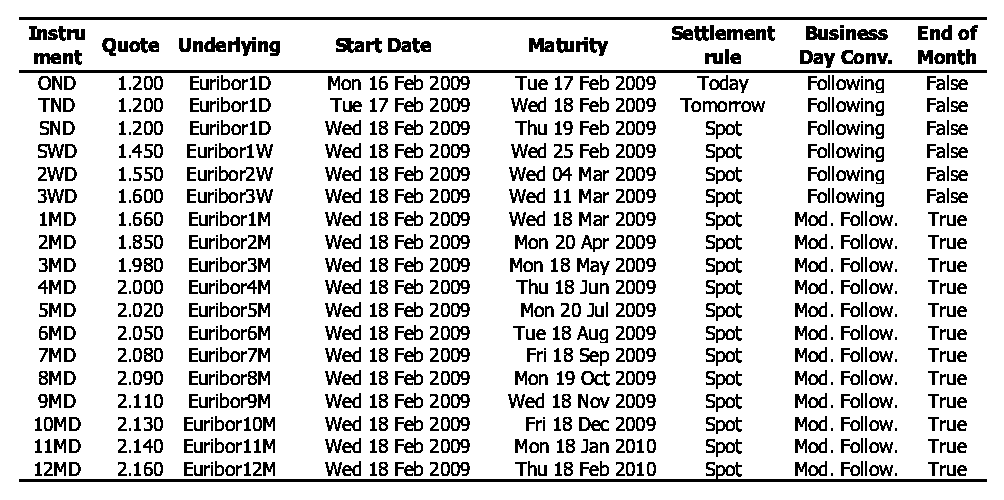
\includegraphics[scale=0.8]{../figures/FigMktDepos}
\caption{EUR Deposit strip. Source: Reuters page KLIEM, 16 Feb. 2009.}
\label{fig:Deposits}
\end{figure}

\subsection{Forward Rate Agreements (FRAs)}
\label{sec:FRA}
\begin{figure}[tbp]
\centering
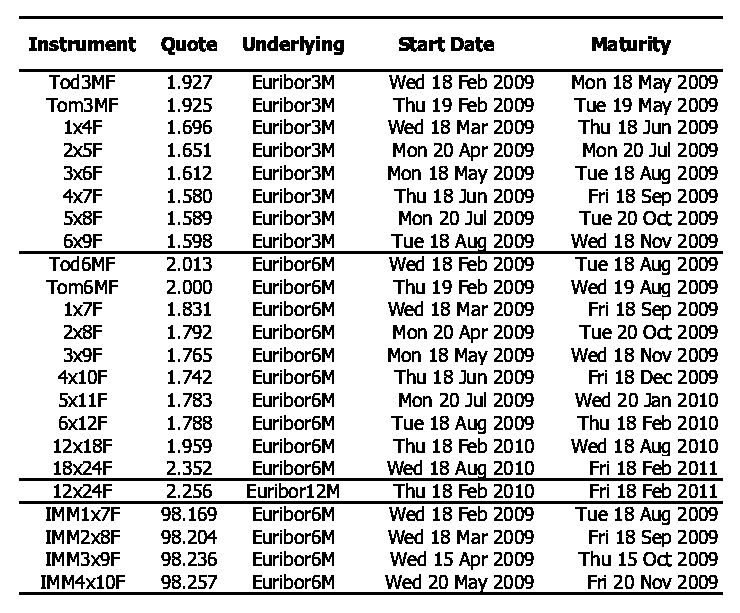
\includegraphics[scale=0.9]{../figures/FigMktFRA}
\caption{EUR FRA strips on Euribor3M, Euribor6M, and Euribor12M. Source: Reuters page ICAPSHORT2, 16 Feb. 2009.}
\label{fig:FRA}
\end{figure}
FRA contacts are forward starting Deposits. For instance the 3x9 FRA is a six months Deposit starting three months forward.
\par
The EUR market quotes standard plain vanilla FRA strips with different forward start dates (i.e. the start date of the forward Depo), calculated with the same convention used for the end date of Deposits. So FRAs do concatenate exactly, e.g. the 6x9 FRA starts when the preceding 3x6 FRA ends. The underlying forward rate fixes two working days before the forward start date.
In fig. \ref{fig:FRA} we report the four FRA strips on 3M, 6M, and 12M Euribor rate quoted in Reuters page ICAPSHORT2.
\par
Market FRAs provide direct empirical evidence that a single curve cannot be used to estimate forward rates with different tenors. We can observe in fig. \ref{fig:FRA} that, for instance, the level of the market 1x4 FRA3M (spanning from 18th March to 18th June, $\tau_{F,1x4} = 0.25556$) was $F_{1x4}^{mkt} = 1.696\%$, the level of market 4x7 FRA3M (spanning from 18th June to 18th September, $\tau_{F,4x7} = 0.25556$) was $F_{4x7}^{mkt}=1.580\%$. If one would compound these two rates to obtain the level of the implied 1x7 FRA6M (spanning from 18th March to 18th September, $\tau_{F,1x7} = 0.50556$) would obtain
\begin{eqnarray}
F_{1x7}^{implied}
&=& \frac{
    \left(1 + F_{1x4}^{mkt}\tau_{F,1x4}\right) \times
    \left(1 + F_{4x7}^{mkt}\tau_{F,4x7}\right) - 1.0}
    {\tau_{F,1x7}} = 1.641\%,
\label{eqn:FRAarbitrage}
\end{eqnarray}
while the market quote for the $1x7$ FRA6M was $F_{1x7}^{mkt}=1.831\%$, 19 basis point larger. As discussed in section \ref{sec:Pricing}, the difference is the liquidity/default risk premium seen by the market in post credit crunch times.
\par
Market FRAs on $x$-tenor Euribor can be selected, together with the corresponding Depos, as bootstrapping instruments for the construction of the short term structure section of the yield curve $\mathcal{C}_x$.
If $F_x\left(t;T_{i-1},T_i\right)$ is the i-th Euribor forward rate resetting at time $T_{i-1}$ with tenor $x=T_i-T_{i-1}$ months associated to the i-th FRA with maturity $T_i$, the implied discount factor at time $T_i$ is obtained by eq. (\ref{eqn:FwdRate}) as
\begin{equation}
P_x\left(t_0,T_i\right) = \frac{P_x\left(t_0,T_{i-1}\right)}{1+F_{x}\left(t_0;T_{i-1},T_{i}\right)\tau_F\left(T_{i-1},T_{i}\right) },\quad t_0<T_{i-1}<T_i,
\label{eqn:FRA}
\end{equation}
where $\tau_F$ is given by eq. (\ref{eqn:yfFRA}). The expression (\ref{eqn:FRA}) above can be used to bootstrap the yield curve $\mathcal{C}_x$ at point $T_i$ once point $T_{i-1}$ is known.
Notice that FRAs collapse to Depos for shrinking $T_{i-1}-t_0$
\begin{equation}
\lim_{T_{i-1} \to t_0}F_{x}\left(t_0;T_{i-1},T_{i}\right) = R^{Depo}_x\left(t_0,T_i\right),
\end{equation}
and eq. (\ref{eqn:FRA}) reduces to eq. (\ref{eqn:Deposit}).
\par

\subsection{Futures}
\label{sec:Futures}
Interest Rate Futures are the exchange-traded contracts equivalent to the over-the-counter FRAs. While FRAs have the advantage of being more customizable, Futures are highly standardized contracts. In the EUR market the most common contracts (so called \emph{IMM}\footnote{International Money Market of the Chicago Mercantile Exchange.} \emph{Futures}) insist on Euribor3M and expire every March, June, September and December (IMM dates). They fix the third Wednesday of the maturity month, the last trading day being the preceding Monday (because of the two days of settlement). Notice that  such date grid is not regular: if $S_i$ is the maturity date of the \textit{i-th} Futures, then $S_i$ and $T_i$, such that $\tau_F\left(S_i,T_i\right)=3M$, are the underlying FRA3M start and end dates, respectively, and, in general, $T_i\neq S_{i+1}$.
There are also so called \emph{serial Futures}, expiring in the upcoming months not covered by the quarterly Futures. Any profit and loss is regulated through daily marking to market (so called \emph{margining process}).
\par
Such standard characteristics reduce the credit risk and the transaction costs, thus enhancing a very high liquidity. The first front contract is the most liquid interest rate instrument, with longer expiry contracts having very good liquidity up to the 8th-12th contract. Also the first serial contract is quite liquid, especially when it expires before the front contract.
\par
In fig. \ref{fig:Futures3M} we report the quoted Futures strip on 3M Euribor rate up to 3 years maturity. As we can see, Futures are quoted in terms of prices instead of rates, the relation being
\begin{equation}
P^{Fut}_x\left(t_0,S_i,T_i\right) = 100 - R^{Fut}_x\left(t_0,S_i,T_i\right),
\label{eqn:FuturePriceRate}
\end{equation}
Because of their daily marking to market mechanism Futures do not have the same payoff of FRAs (including an unitary discount factor): an investor long a Futures contract will have a loss when the Futures price increases (and the Futures rate decreases) but he will finance such loss at lower rate; viceversa when the Futures price decreases the profit will be reinvested at higher rate. This means that the volatility of the forward rates and their correlation to the spot rates have to be accounted for, hence a \emph{convexity adjustment} is needed to convert the rate $R^{Fut}_x$ implied in the Futures price to its corresponding forward rate $F_x$,
\begin{equation}
F_x\left(t_0,S_i,T_i\right) = R^{Fut}_x\left(t_0,S_i,T_i\right)-C_x\left(t_0,S_i,T_i\right)
\label{eqn:fwdfromfutureprice}
\end{equation}
(see e.g. ref. \cite{JacKaw05}).
In other words, the trivial unit discount factor implied by daily margination introduces a pricing measure mismatch with respect to the corresponding FRA case that generates a volatility-correlation dependent convexity adjustment (see e.g. ch. 12 in ref. \cite{BriMer06}).
\begin{figure}[tbp]
\centering
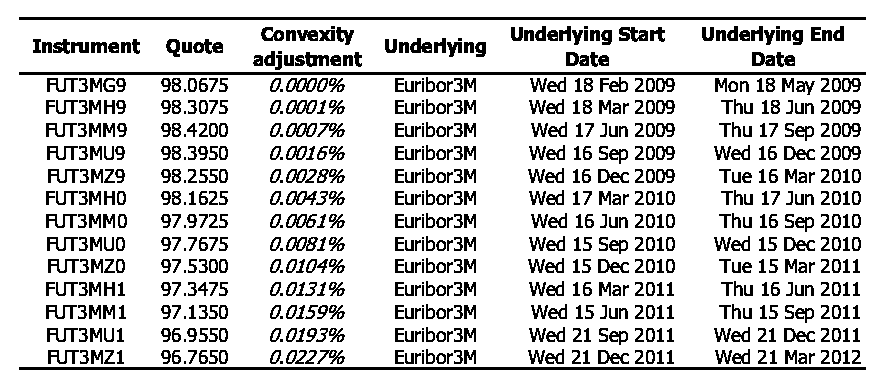
\includegraphics[scale=0.9]{../figures/FigMktFut3M}
\caption{EUR Futures on Euribor 3M. The first serial contract (where \textquotedblleft G9\textquotedblright stands for Feb. 09 expiry) and three IMM sets (where \textquotedblleft H\textquotedblright, \textquotedblleft M\textquotedblright, \textquotedblleft U\textquotedblright and \textquotedblleft Z\textquotedblright stand for March, June, September and December expiries, respectively) are displayed. Source: Reuters page 0\#/FEI, 16 Feb. 2009. In column 3 are reported the corresponding convexity adjustments, calculated as discussed in the text.}
\label{fig:Futures3M}
\end{figure}
\begin{table}[tbp]
\begin{tabular}{lc}
\midrule
HW parameter   & Value \\
\midrule
Mean reversion & 0.03  \\
Volatility & 0.709\%   \\
\midrule
\end{tabular}
\caption{Hull-White parameters values for Futures3M convexity adjustment at 16 Feb. 2009.}
\label{tab:FuturesConAdy}
\end{table}
\par
The calculation of convexity adjustment thus requires a model for the evolution of the rates.  While advanced approaches are available in literature (see e.g. refs. \cite{JacKaw05}, \cite{PitRen06}, \cite{BriMer06}), a standard practitioners' recipe is given in ref. \cite{KirNov1997}, based on a simple short rate 1 factor Hull \& White model \cite{HulWhi1990}. This approach has been used in fig. \ref{fig:Futures3M} to calculate the adjustments, using the  Hull-White parameters values given in table \ref{tab:FuturesConAdy}.
\par
Market Futures on $x$-tenor Euribor can be selected as bootstrapping instruments for the construction of short-medium term structure section of the yield curve $\mathcal{C}_x$.
Notice that Futures contracts have expiration dates gradually shrinking to zero and as such they generate rolling pillars that periodically jumps and overlap the fixed Depo and FRA pillars. Hence some \emph{priority} rule must be used in order to decide which instruments must be excluded from the bootstrapping procedure.
\par
Given the i-th Futures market quote $P^{Fut}_x\left(t_0,S_i,T_i\right)$ with underlying FRA maturity $T_i$, the implied discount factor at time $T_i$ is obtained by eqs. (\ref{eqn:FRA}), (\ref{eqn:FuturePriceRate}) and (\ref{eqn:fwdfromfutureprice}) as
\begin{equation}
P_x\left(t_0,T_i\right)
=   \frac{P_x\left(t_0,T_{i-1}\right)}
         {1+\left[R^{Fut}_x\left(t_0,S_i,T_i\right) -
          C_x\left(t_0,S_i,T_i\right)\right]
          \tau_F\left(S_i,T_i\right)},
\label{eqn:FuturesBootstrap}
\end{equation}
where $\tau_F$ is given by eq. (\ref{eqn:yfFRA}). The expression above can be used to bootstrap the yield curve $\mathcal{C}_x$ at point $T_i$ once point $S_i$ is known.


\subsection{Swaps}
\label{sec:Swap}
Interest rate Swaps are Over-The-Counter (OTC) contracts in which two counterparties agree to exchange fixed against floating rate cash flows. These payment streams are called fixed and floating leg of the Swap, respectively.
\par
The EUR market quotes standard plain vanilla Swaps starting at spot date with annual fixed leg versus floating leg indexed to x-months Euribor rate payed with x-months frequency. Such Swaps can be regarded as portfolioS of FRA contracts (the first one being actually a Deposit). The day count convention for the quoted (fair) swap rates is \emph{30/360 (bond basis)} \cite{ISDA}.
In figures \ref{fig:Swaps6M}, \ref{fig:SwapsIMM} and \ref{fig:Swaps1M} we report the quoted Swaps strips on 6M, 3M and 1M Euribor rates, respectively.
\begin{figure}[tbp]
\centering
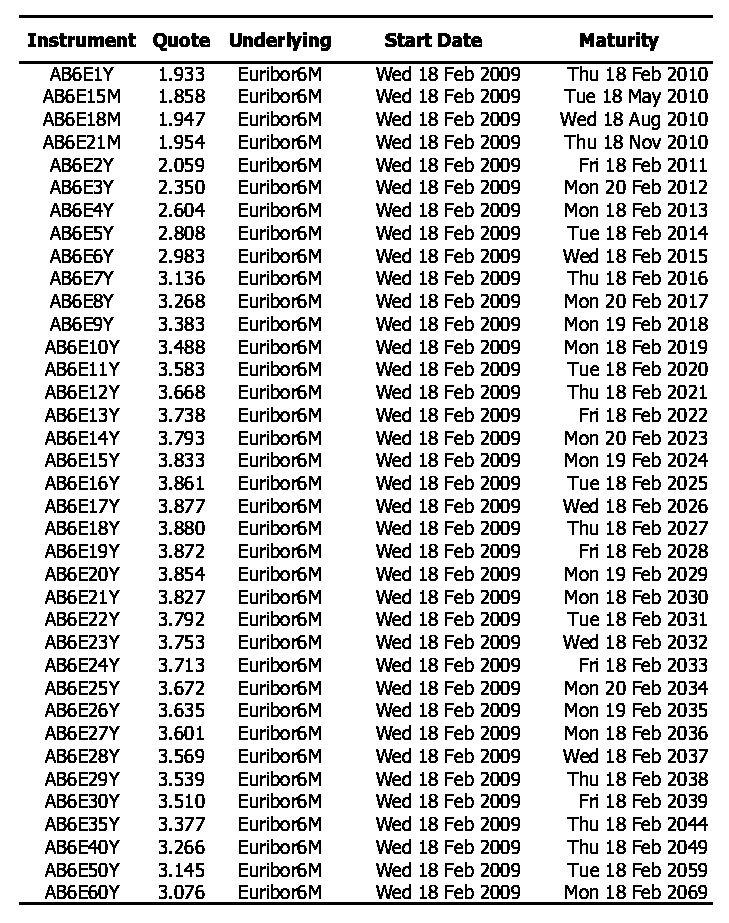
\includegraphics[scale=0.9]{../figures/FigMktSwaps6M}
\caption{EUR Swaps on Euribor6M. The codes \textquotedblleft AB6E$n$\textquotedblright in col. 1 label swaps receiving annually a fixed rate and paying semi-annually a floating rate on Euribor6M with maturity in $n$ months/years. Source: Reuters page ICAPEURO, 16 Feb. 2009.}
\label{fig:Swaps6M}
\end{figure}

\begin{figure}[tbp]
\centering
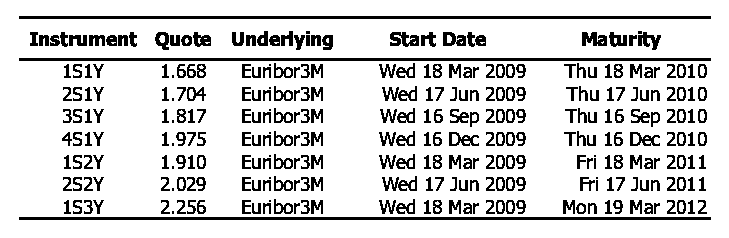
\includegraphics[scale=0.9]{../figures/FigMktSwapsIMM}
\caption{EUR IMM Swaps on Euribor3M. The codes \textquotedblleft $m$S$n$Y\textquotedblright in col. 1 label $m=$ Mar., Jun., Sep. and Dec. IMM starting swaps receiving annually a fixed rate and paying quarterly a floating rate on Euribor3M with maturity in $n=1,2,3$ years. Source: Reuters page ICAPSHORT2, 16 Feb. 2009.}
\label{fig:SwapsIMM}
\end{figure}

\begin{figure}[tbp]
\centering
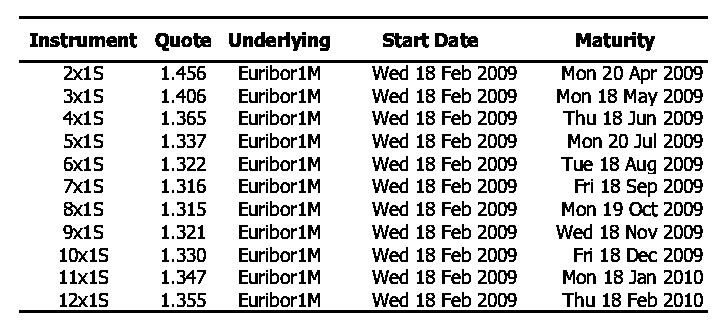
\includegraphics[scale=0.9]{../figures/FigMktSwaps1M}
\caption{EUR Swaps on Euribor1M. The codes \textquotedblleft $n$x1S\textquotedblright in col. 1 label $n$-months maturity swaps receiving a single fixed rate at maturity and paying monthly a floating rate on Euribor1M. Source: Reuters page ICAPSHORT2, 16 Feb. 2009.}
\label{fig:Swaps1M}
\end{figure}

\par
Market Swaps on $x$-tenor Euribor can be selected as bootstrapping instruments for the construction of the medium-long term structure section of the yield curve $\mathcal{C}_x$.
By setting $T_0=S_0=t=t_0$ and $T_n=S_m=T_i=S_j$ in equation (\ref{eqn:SwapRateFwd}) we obtain, for the swap rate
$S_x\left(t_0,T_i\right):= S_x\left(t_0;t_0,...,S_j;t_0,...,T_i\right)$
quoted for maturity $T_i=S_j$,
\begin{multline}
S_x\left(t_0,T_i\right)
= \frac{\sum\limits_{\alpha=1}^j P_x\left(t_0,S_\alpha\right) \tau_F\left(S_{\alpha-1},S_\alpha\right)
F_x\left(t_0;S_{\alpha-1},S_\alpha\right)}
{A_x\left(t_0,T_i\right)} \\
= \left[\sum\limits_{\alpha=1}^{j-1} P_x\left(t_0,S_\alpha\right) \tau_F\left(S_{\alpha-1},S_\alpha\right)
F_x\left(t_0;S_{\alpha-1},S_\alpha\right)\right. \\
+ P_x\left(t_0,S_{j-1}\right) - P_x\left(t_0,T_i\right)\bigg]
\frac{1}{A_x\left(t_0,T_{i-1}\right)+\tau_S\left(T_{i-1},T_i\right)P_x\left(t_0,T_i\right)},
\label{eqn:SwapRateMkt}
\end{multline}
where the last discount factor $P_x\left(t_0,T_i\right)$ has been separated in the second line, the annuity $A_x\left(.\right)$ is given by eq. (\ref{eqn:Annuity}), and $\tau_S$ is given by
\begin{equation}
\tau_S\left(T_1,T_2\right) := \tau\left[T_1,T_2;30/360 (bond basis)\right].
\end{equation}
Notice that in eq. \ref{eqn:SwapRateMkt} above we have not used the telescopic property of the summation (see the discussion closing section \ref{sec:Math}). Eq. \ref{eqn:SwapRateMkt} can be inverted to find $P_x\left(t_0,T_i\right)$ as
\begin{multline}
P_x\left(t_0,T_i\right)
= \left[\sum\limits_{\alpha=1}^{j-1} P_x\left(t_0,S_\alpha\right)\tau_F\left(S_{\alpha-1},S_\alpha\right)
F_x\left(t_0;S_{\alpha-1},S_\alpha\right)\right. \\
+ P_x\left(t_0,S_{j-1}\right)
- S_x\left(t_0,T_i\right)A_x\left(t_0,T_{i-1}\right)\bigg]
\frac{1}{1+S_x\left(t_0,T_i\right)\tau_S\left(T_{i-1},T_i\right)}.
\label{eqn:SwapBootstrap}
\end{multline}
The expression (\ref{eqn:SwapBootstrap}) above can be used, in principle, to bootstrap the yield curve $\mathcal{C}_x$ at point $T_i=S_j$ once the curve points at $\left\{T_1,...,T_{i-1}\right\}$ and $\left\{S_1,...,S_{j-1}\right\}$ are known.
In practice, since the fixed leg frequency is annual and the floating leg frequency is given by the underlying Euribor rate tenor, we have that
$\left\{T_1,...,T_i\right\} \subseteq \left\{S_1,...,S_j=T_i\right\}$ for any given fixed leg date $T_i$. Hence some points between $P_x\left(t_0,T_{i-1}\right)$ and $P_x\left(t_0,T_i\right)$ in eq. (\ref{eqn:SwapBootstrap}) may be unknown and one must resort to interpolation and, in general, to a numerical solution.
For example the bootstrap of Euribor6M curve $\mathcal{C}_{6M}$ from 9Y to 10Y knots using the quotation $S_x\left(t_0,T_{10}\right)=3.488\%$ in fig. \ref{fig:Swaps6M} is given by
\begin{multline}
P_x\left(t_0,T_{10}\right)
= \left[\sum\limits_{\alpha=1}^{19} P_x\left(t_0,S_\alpha\right)\tau_F\left(S_{\alpha-1},S_\alpha\right)
F_x\left(t_0;S_{\alpha-1},S_\alpha\right)\right. \\
+ P_x\left(t_0,S_{19}\right)
- S_x\left(t_0,T_{10}\right)A_x\left(t_0,T_{9}\right)\bigg]
\frac{1}{1+S_x\left(t_0,T_{10}\right)\tau_S\left(T_{9},T_{10}\right)},
\label{eqn:SwapBootstrapExample}
\end{multline}
where $\mathbf{T}=\left\{T_1,...,T_{10}\right\}$, $\mathbf{S}=\left\{S_1,...,S_{20}\right\}$, $T_9=S_{18}=9Y, S_{19}=9.5Y, T_{10}=S_{20}=10Y$.
Since $P_x\left(t_0,S_{19}\right)$ in eq. \ref{eqn:SwapBootstrapExample} above is unknown, it must be interpolated between $P_x\left(t_0,T_9\right)$ (known) and $P_x\left(t_0,T_{10}\right)$ (unknown).
\par
We thus see, as anticipated in the introduction, that interpolation is already used during the bootstrapping procedure, not only after that.

\subsection{Basis Swaps}
\label{sec:BasisSwaps}
Interest rate (single currency) Basis Swaps are floating vs floating swaps admitting underlying rates with different tenors.
\par
The EUR market quotes standard plain vanilla Basis Swaps as portfolios of two swaps with the same fixed legs and floating legs paying Euribor xM and yM, e.g. 3M vs 6M, 1M vs 6M, 6M vs 12M, etc.
In fig. \ref{fig:BasisSwaps} we report three quoted Basis Swaps strips.
The quotation convention is to provide the difference (in basis points) between the fixed rate of the higher frequency swap and the fixed rate of the lower frequency swap. At the moment such difference is positive and decreasing with maturity, reflecting the preference of market players for receiving payments with higher frequency (e.g. 3M instead of 6M, 6M instead of 12M, etc.) and shorter maturities.
%NOTA: lo swap1M a 1Y implicito nei basis vale 1.933-0.551 = 1.382 mentre lo swap1M 1Y quotato (12x1S) vale 1.355, 2.7 bps di differenza...illiquidit� ?
\begin{figure}[tbp]
\centering
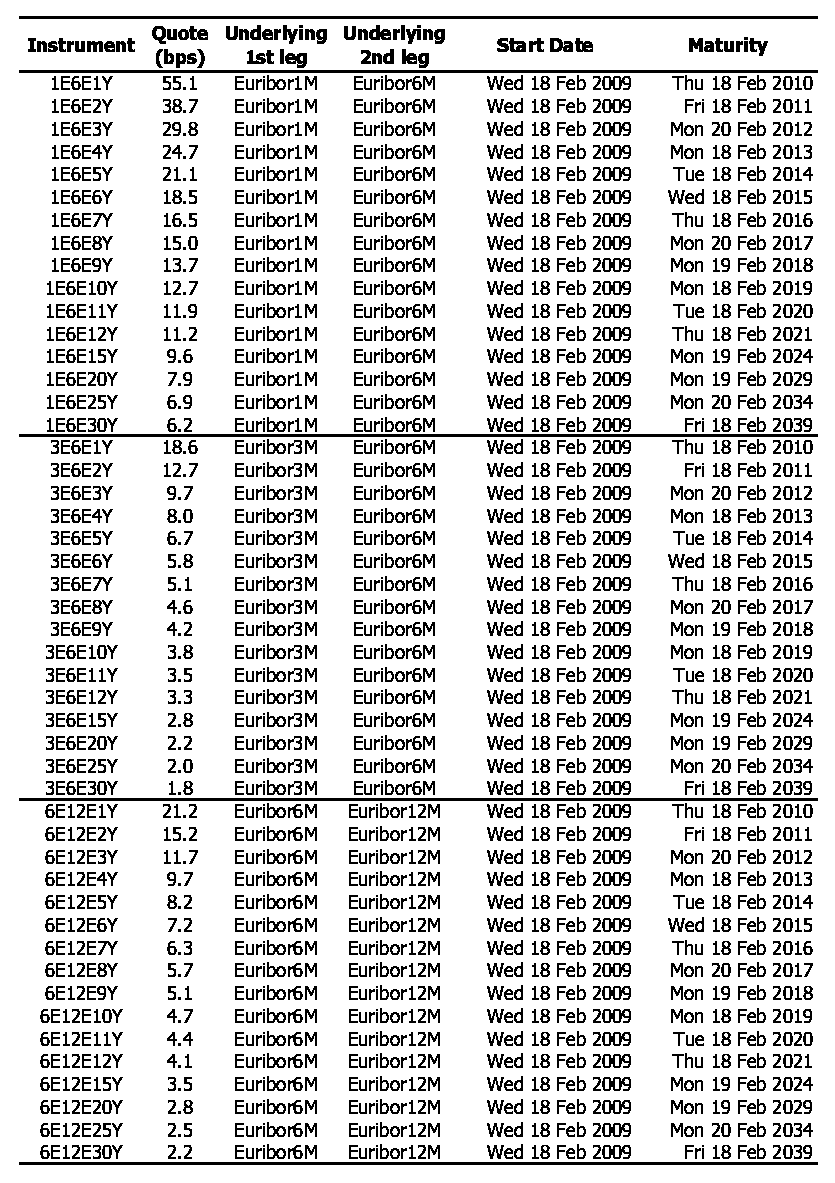
\includegraphics[scale=0.9]{../figures/FigMktBasis}
\caption{EUR Basis Swaps. The codes \textquotedblleft $x$E$y$E$n$Y\textquotedblright in col. 1 label basis swaps receiving Euribor $x$M and paying Euribor $y$M plus basis spread with $n$ years maturity. Source: Reuters page ICAPEUROBASIS, 16 Feb. 2009.}
\label{fig:BasisSwaps}
\end{figure}

\begin{figure}[tbp]
\centering
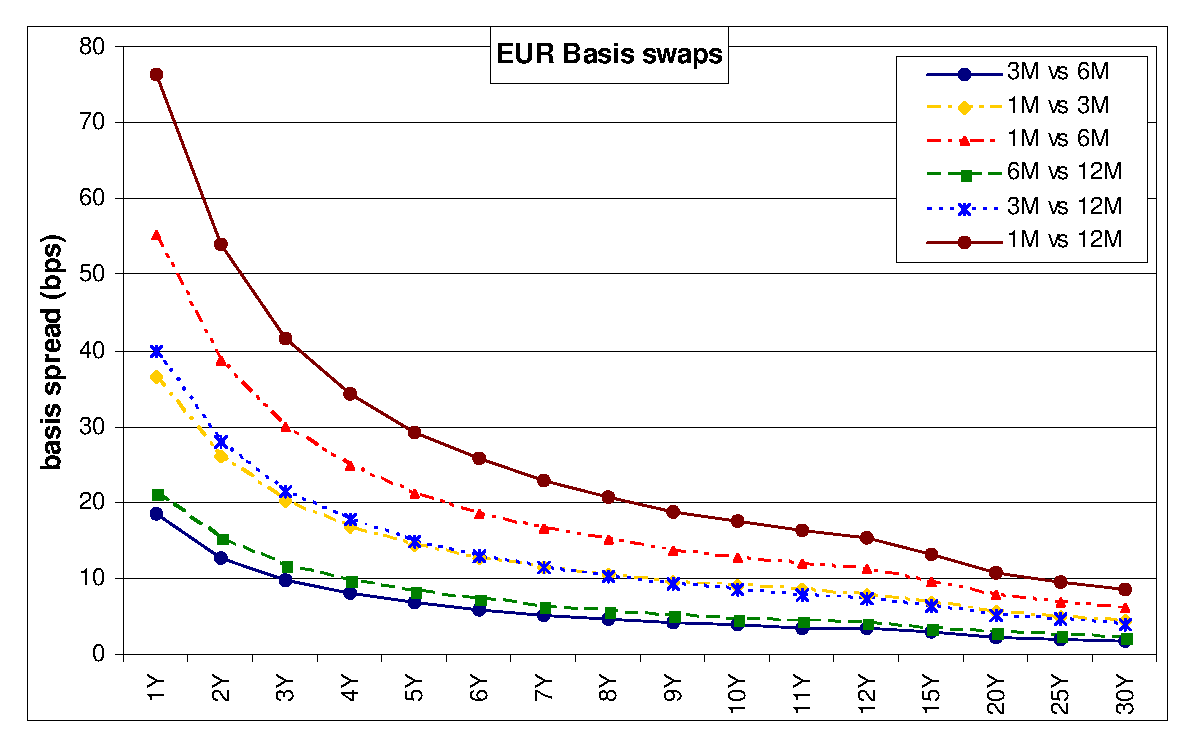
\includegraphics[scale=0.65]{../figures/FigMktBasisGraph}
\caption{EUR Basis spreads from fig. \ref{fig:BasisSwaps}. The spreads not explicitly quoted there have been deduced using eq. (\ref{eqn:BasisSwap}).}
\label{fig:BasisSwapsGraph}
\end{figure}
\par
Basis swaps are a fundamental element for long term multi-curve bootstrapping, because, starting from the quoted Swaps on Euribor 6M (fig. \ref{fig:Swaps6M}), they allow to imply levels for non-quoted Swaps on Euribor 1M, 3M, and 12M, to be selected as bootstrapping instruments for the corresponding yield curves construction.
If $\Delta_{x,6M}\left(t_0,T_i\right)$ is the quoted basis spread for a basis swap receiving Euribor $x$M and paying Euribor 6M plus spread for maturity $T_i$, we simply have
\begin{equation}
S_x\left(t_0,T_i\right) = S_{6M}\left(t_0,T_i\right) + \Delta_{x,6M}\left(t_0,T_i\right),
\label{eqn:BasisSwap}
\end{equation}
with the obvious caveat that
$\Delta_{6M,x}\left(t_0,T_i\right) = - \Delta_{x,6M}\left(t_0,T_i\right)$. In fig. \ref{fig:BasisSwapsGraph} we report all the possible basis combinations obtained from fig. \ref{fig:BasisSwaps}.
Notice that basis swaps in fig. \ref{fig:BasisSwaps} are quoted up to 30 years, while swaps on Euribor6M in fig. \ref{fig:Swaps6M} are quoted up to 60 years. Thus the bootstrapping of yield curves different from $\mathcal{C}_{6M}$ over 30 years maturity requires extrapolation of basis swap quotations. In the present market conditions, such extrapolation is not particularly critical, given the smooth and monotonic long term shape of the basis curves in fig. \ref{fig:BasisSwaps}.

\subsection{The Role of Interpolation}
\label{sec:Interp}
The interpolation scheme we choose for the given parametrization determines how reasonable the yield curve will be. For instance, linear interpolation of discount factors is an obvious but extremely poor choice. Linear interpolation of zero rates or log-discounts are popular choices leading to stable and fast bootstrapping procedures, but unfortunately they produce horrible forward curves, with a sagsaw or piecewise-constant shape (see e.g. \cite{HagWes06}, \cite{HagWes08} for a review of available interpolation schemes).
We show in fig. \ref{fig:Interpolations} one examples of such poor interpolation schemes. While zero curves (upper panel) display similar smooth behaviors, simple visual inspection of forward curves (lower panel) reveals different non-smooth behaviors, with oscillations larger than 100 basis points.
Such discontinuities in the forward curves correspond to angle points in the zero curves (as pointed out in section \ref{sec:Math}), generated by linear interpolation that forces them to suddenly \textquotedblleft turn\textquotedblright around a market point.
Notice that only the most liquid Swaps from fig. \ref{fig:Swaps6M}, with maturities 3-10, 12, 15, 20, 25 and 30 years have been included in the bootstrapping of curve $\mathcal{C}_{6M}$. Often the remaining less liquid quotations for 11, 13, 14, 16-19, 21-24, 26-29 years maturity are included in the linear interpolations schemes to reduce the amplitude of the forward curve oscillations. The same can be done for longer maturities using interpolated quotes on the 30, 40, 50 and 60 years market pillars.

\begin{figure}[tbp]
\centering
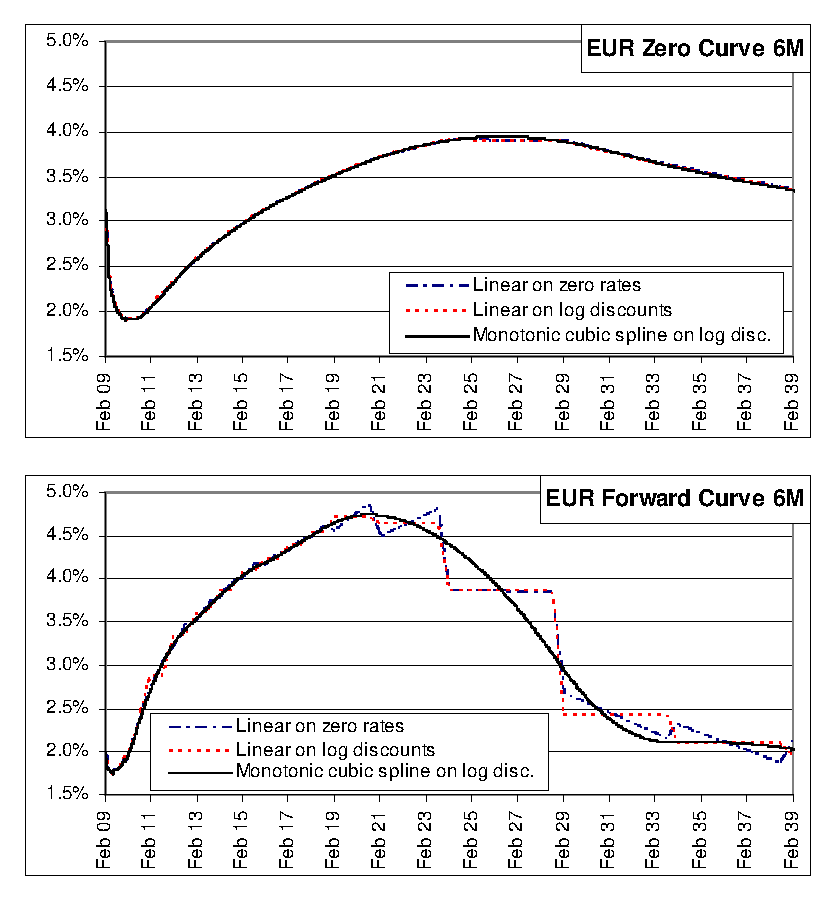
\includegraphics[scale=0.95]{../figures/FigInterpolations}
\caption{Examples of \emph{bad} (but very popular!) interpolation schemes. Upper panel: different zero curves display similar smooth behaviors. Lower panel: forward curves reveals different non-smooth behaviors, with oscillations larger than 100 basis points. The smooth monotonic cubic spline interpolation on log-discounts (continuous black line) of fig. \ref{FigYC6M} is shown as a benchmark.}
\label{fig:Interpolations}
\end{figure}

\begin{figure}[tbp]
\centering
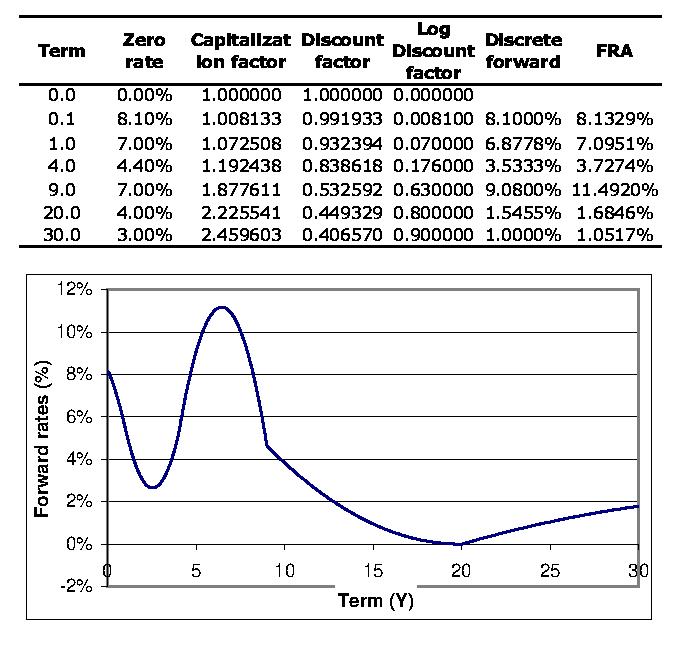
\includegraphics[scale=0.9]{../figures/FigInterpolationHagan}
\caption{Example of nasty curve taken from ref. \cite{HagWes06} (p. 98 and fig. 2, bottom right panel). Upper panel: the example curve. Lower panel: the forward curve obtained through Hyman monotonic cubic spline \cite{Hym1983} applied on log-discounts. The forward rate at 20Y is null but no negative rates appear.}
\label{fig:InterpolationHagan}
\end{figure}

\par
In fig. \ref{fig:Interpolations} the monotonic cubic spline interpolation on log-discounts is shown too, clearly ensuring a smooth and financially sound behavior of the forward curve.
The choice of cubic interpolations is a very delicate issue. Simple splines (see e.g. \cite{PreTeu07}) suffer of well-documented problems such as spurious inflection points, excessive convexity, and lack of locality after input price perturbations (distributed sensitivities). Recently, Andersen \cite{And07} has addressed these issues through the use of shape-preserving splines from the class of generalized tension splines, while Hagan and West \cite{HagWes06}-\cite{HagWes08} have developed a new scheme based on positive preserving forward interpolation.
We found the classic Hyman monotonic cubic filter \cite{Hym1983} applied to spline interpolation of log-discounts to be the easiest and best approach: its monotonicity ensures non-negative forward curves and actually remove most of the unpleasant waviness. Notice that the Hyman filter can be applied to any cubic interpolants: this helps to address the non-locality of spline using alternative more local cubic interpolations. In fig. \ref{fig:InterpolationHagan} we show an example of particularly nasty curve taken from Hagan and West \cite{HagWes06} (p. 98 and fig. 2, bottom right panel). The forward curve obtained through Hyman monotonic cubic spline \cite{Hym1983} applied on log discounts (lower panel) is always non negative (there is a unique minimum at 20Y).
\par
A peculiarity of using non-local interpolation inside the bootstrapping procedure is that the shape of the already bootstrapped part of the curve is altered by the addition of further pillars. This is usually remedied by cycling in iterative fashion: after a first bootstrap, which might even use a local interpolation scheme and build up the pillar grid one point at time, the resulting complete grid is altered one pillar at time using again the same bootstrapping algorithm, until convergence is reached. The first cycle can be even replaced by a good grid guess, the most natural one being just the grid previous state in a dynamically changing environment.
\par
We stress that the focus on smooth discrete forward rate is the key point of state-of-the-art bootstrapping. For even the best interpolation schemes to be effective the forward rate curve must be smooth, i.e. any jump must be removed, and added back only at the end of the smooth curve construction. The most relevant jump in forward rates is the so-called turn of year effect, discussed in the next section.

\subsection{The Turn of Year Effect}
\label{sec:TOY}
In the interest rate market the turn of year effect is a jump normally observed in market quotations of rates spanning across the end of a year. In fig. \ref{fig:Euribor1M} we display the historical series of Euribor1M in the window October 2007 - February 2009.
The 2007 turn of year jump (64 bps) is clearly visible on 29th Nov. 2007 (left rectangle), just when the spot starting 1M tenor rate spans the end of 2007, with rates reverting toward the previous levels one month later.
The 2008 turn of year jump on 27th Nov. 2008 (22 bps, right oval) is partially hidden by the high market volatility realized in that period. Viceversa in lower volatility regimes even the much smaller \textquotedblleft end of semester effect\textquotedblright may be observable, as seen on 29th of May 2008 (9 bps, middle rhombus).
\par
In the EUR market the larger jump is observed the last working day of the year (e.g. 31th December) for the Overnight Deposit maturing the first working day of the next year (e.g. 2nd January).
The same happens for the Tomorrow Next and Spot Next Deposits one and two business days before, respectively (e.g. 30th and 29th December).
Other instruments with longer underlying rate tenors display smaller jumps when their maturity crosses the same border: for instance, the 1M Deposit quotation jumps 2 business days before the 1st business day of December; the 12M Deposits always include a jump except 2 business days before the end of the year (due to the end of month rule); the December IMM Futures always include a jump, as well as the October and November serial Futures; 2Y Swaps always include two jumps; etc.
The effect is generally observable at the first two ends of year and becomes negligible at the following crosses.
\par
The decreasing jump with increasing underlying rate tenor can be easily understood once we distinguish between jumping rates and non-jumping rates.
For instance, we may think to the 1M Deposit as a weighted average of 22 (business days in one month) overnight rates (plus a basis). If such Depo spans an end of year, there must be a single overnight rate, weighting 1/22th, that crosses that end of year and displays the jump, while the others do not. Considering rates with longer tenors, there are still single jumping overnight rates, but with smaller weights. Hence longer deposits/FRAs display smaller jumps. The same holds for Swaps, as portfolios of Depos/FRAs.
\par
From a financial point of view, the turn of year effect is due to the increased search for liquidity by financial institutions just after the periodic balance sheet strikes.
%NOTA: AMPLIARE QUESTA SPIEGAZIONE
\begin{figure}[tbp]
\centering
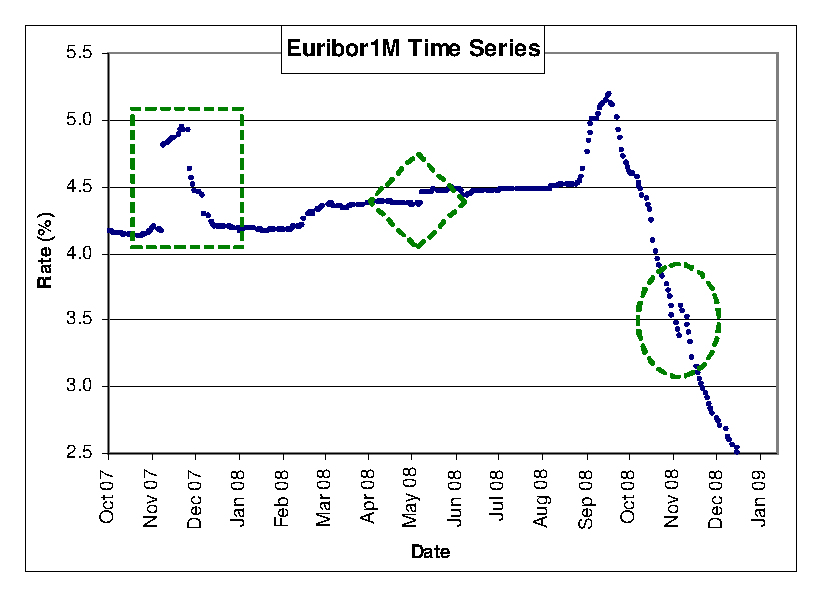
\includegraphics[scale=0.95]{../figures/FigEuribor1M}
\caption{Turn of year effect on Euribor1M. The historical time series in the Oct. 2007 - Feb 2009 window is displayed. Three jumps can be identified: the 2007 turn of year (29th Nov. 2007, 64 bps, left rectangle); the 2008 turn of year (27th Nov. 2008, 22 bps, right oval); a smaller \textquotedblleft end of semester effect\textquotedblright (29th May 2008, 9 bps, middle rhombus). Source: Reuters.}
\label{fig:Euribor1M}
\end{figure}
\begin{figure}[tbp]
\centering
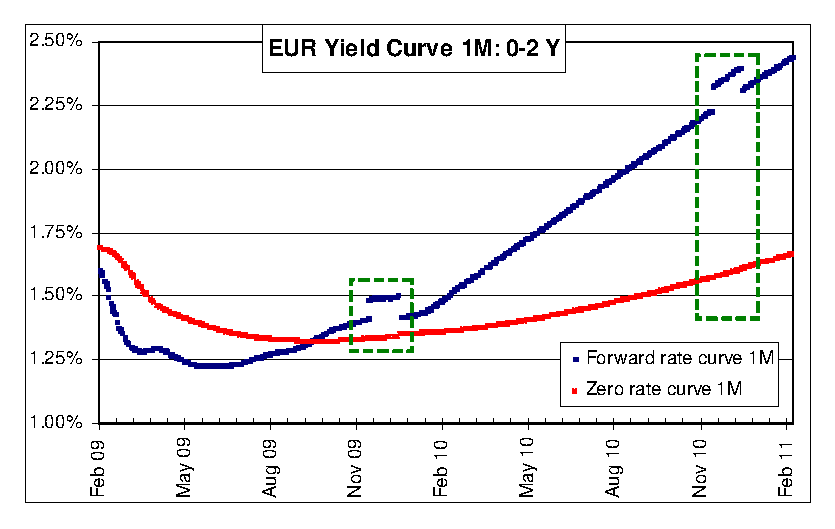
\includegraphics[scale=0.95]{../figures/FigYC1MToY}
\caption{Detail from fig. \ref{FigYC1M}, upper panel, showing the turn of year effect included in the short term bootstrapping of the forward rate curve $\mathcal{C}_{1M}^f$ (blue line). The 2009 and 2010 turn of year jumps are clearly observable (left and right dashed rectangles, respectively). The same jumps are also present in the zero rate curve $\mathcal{C}_{1M}^z$ (red line), but less visible because of the scale (see discussion in the text).}
\label{fig:YC1MToY}
\end{figure}\par
An yield curve term structure up to $N$ years including the turn of year effect should contain, in principle, $N$ discontinuities; in practice essentially the end of the current and the next year can be taken into account.
The effect can be modeled simply through a multiplicative coefficient applied to discount factors, or, equivalently, an additive coefficient applied to zero rates, corresponding to all the dates following a given end of year.
In this way we are allowed to estimate the coefficient using instruments with a given underlying rate tenor (e.g. those on Euribor3M used for $\mathcal C_{3M}$), and to apply it to any other curve $\mathcal C_x$ taking into account the proper weights.
Notice that, as stressed in the previous section, starting from a smooth and continuous yield curve is crucial for correctly take into account the discontinuity at the turn of year.
\par
The jump coefficient can be estimated from market quotations using different approaches:
\begin{itemize}
  \item jump in the 3M Futures strip: the (no-jump) end of year crossing forward is obtained through interpolation of non-crossing forwards; the jump coefficient is given by the difference between the latter and the quoted value. This approach always allows the estimation of the second turn of year. The first turn of year can be obtained only up to the third Wednesday of September, when the corresponding Futures expires. In the period October-December there are no non-crossing Futures to interpolate and the first turn of year should be extrapolated from the second, making the method not robust;
  \item jump in the 6M FRA strip: this is equivalent to the approach above but it allows the estimation of the first turn of year up to June (included);
  \item jump in the 1M Swaps strip: this is equivalent to the approaches above and it allows the estimation of the first turn of year up to November (included);
  \item jump in the FRA strip quoted by brokers each Monday: this approach is valid all year long, but it allows only a discontinuous weekly update.
\end{itemize}
The empirical approaches above, when available at the same time, give estimates in excellent agreement with each other.
\par
A numerical example of application of the methodology discussed above is given in fig. \ref{fig:YC1MToY} (a detail from upper panel of fig. \ref{FigYC1M} reported in section \ref{sec:ImplementResults}), where we display the bootstrapping of the forward and zero rate curves $\mathcal{C}_{1M}^f$ and $\mathcal{C}_{1M}^z$ on Euribor1M.
The 2009 turn of year jump is clearly observable in $\mathcal{C}_{1M}^f$ from 27th Nov. 2009 (+7.5 bps) to 30th Dec. 2009 (-8.6 bps) for Euribor1M rates spot starting on 1st Dec. 2009 and terminating on 4th Dec. 2010.
Also the 2010 turn of year jump is observable in $\mathcal{C}_{1M}^f$ from 29th Nov. 2010 (+9.3 bps) to 30th Dec. 2010 (-8.6 bps) for rates spot starting on 1st Dec. 2010 and terminating on 3rd Dec. 2011.
The jumps are present also in the zero rate curve $\mathcal{C}_{1M}^z$, but they are less observable because of the scale in fig. \ref{fig:YC1MToY}.
We stress that a single turn of the year induces \emph{one} discontinuity in the zero rate and discount curves, and \emph{two} discontinuities in the forward rate curve (remember that the forward rate is given by the ratio of two discounts).
% NOTA: VERIFICARE CURVA DISCOUNT
\par
The yield curve discontinuities induced by the turn of year effect may appear, to a non market-driven reader, a fuzzy effect broking the desired yield curve smoothness. On the contrary, we stress that they are neither a strangeness of the market quotations nor an accident of the bootstrapping, but correspond to true and detectable financial effects that should be included in any yield curve used to mark to market interest rate derivatives.


\section{Implementation and Examples of Bootstrapping}
\label{sec:ImplementResults}
Given the methodology discussed in the previous sections, we are able to bootstrap four yield curves $\mathcal{C}_{1M}$, $\mathcal{C}_{3M}$, $\mathcal{C}_{6M}$, $\mathcal{C}_{12M}$ on Euribor 1M, 3M, 6M and 12M, respectively.
In the four figures \ref{FigYC1M}, \ref{FigYC3M}, \ref{FigYC6M} and \ref{FigYC12M} below we show an example of bootstrapping using our personal selection of the market data discussed in sections \ref{sec:Depo}-\ref{sec:BasisSwaps}. Only the forward curves are displayed, being the most significative bootstrapping test as discussed in section \ref{sec:Interp}.
The scales are the same across all figures, allowing a general comparison. The maximum maturity reported is 30 years, according to the basis swaps quotations (see fig. \ref{fig:BasisSwaps}). As discussed in section \ref{sec:BasisSwaps}, while for the $\mathcal{C}_{6M}$ curve swaps market data are available up to 60 years (see fig. \ref{fig:Swaps6M}), the bootstrapping of other curves
over 30 years maturity would require extrapolation of basis swap quotations (see figures \ref{fig:BasisSwaps} and \ref{fig:BasisSwapsGraph}).
%NOTA: COMPLETARE DISCUSSIONE GENERALE DELLE CURVE
%curve zero, smoothness, turn of the year, short term structure, instrument selection, mixed upward/downward sloping behavior
\par
The results discussed in this paper have been obtained using the QuantLib framework\footnote{precisely, revision 15931 in the QuantLib SVN repository.}. The basic classes and methods (iterative bootstrapping, interpolations, market conventions, etc.) are implemented in the object oriented C++ QuantLib library \cite{QuantLib}. The QuantLib objects and analytics are exposed to a variety of end-user platforms (including Excel and Calc) through the QuantLibAddin \cite{QuantLibAddin} and QuantLibXL \cite{QuantLibXL} libraries. Market data are retrieved from the chosen provider and real time is ensured by the ObjectHandler in-memory repository \cite{ObjectHandler}.
The full framework described above is available open source. Anyone interested in the topic may download and test the implementation, posting to the QuantLib community forum any comment or suggestion to improve the job.

\begin{figure}[tbp]
\centering
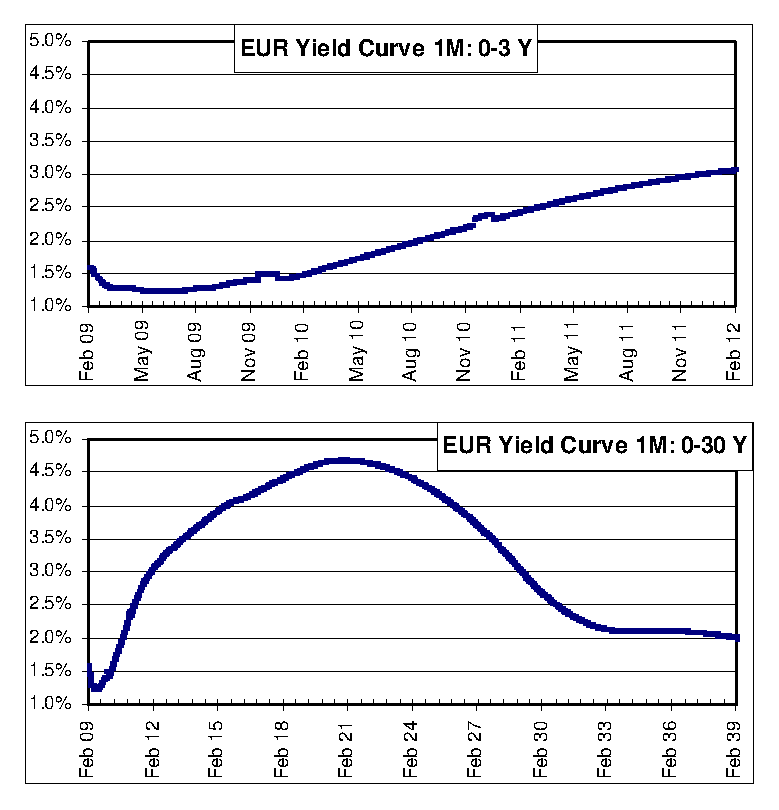
\includegraphics[scale=1.0]{../figures/FigYC1M}
\caption{Forward curve $\mathcal{C}_{1M}^f$ on Euribor1M at 16 Feb. 2009, plotted with 1M-tenor forward rates $F\left( t_{0};t,t+1M,\text{\textit{act/360}}\right)$, $t$ daily sampled and spot date $t_{0}=$ Feb. 18th, 2009. Upper panel: short term structure up to 3 years; lower panel: whole term structure up to 30 years. The two jumps observed in the curve correspond to the two turn of years for 1M tenor forward rates spot starting at 1st Dec. 2009 and 1st Dec. 2010.}
\label{FigYC1M}
\end{figure}

\begin{figure}[tbp]
\centering
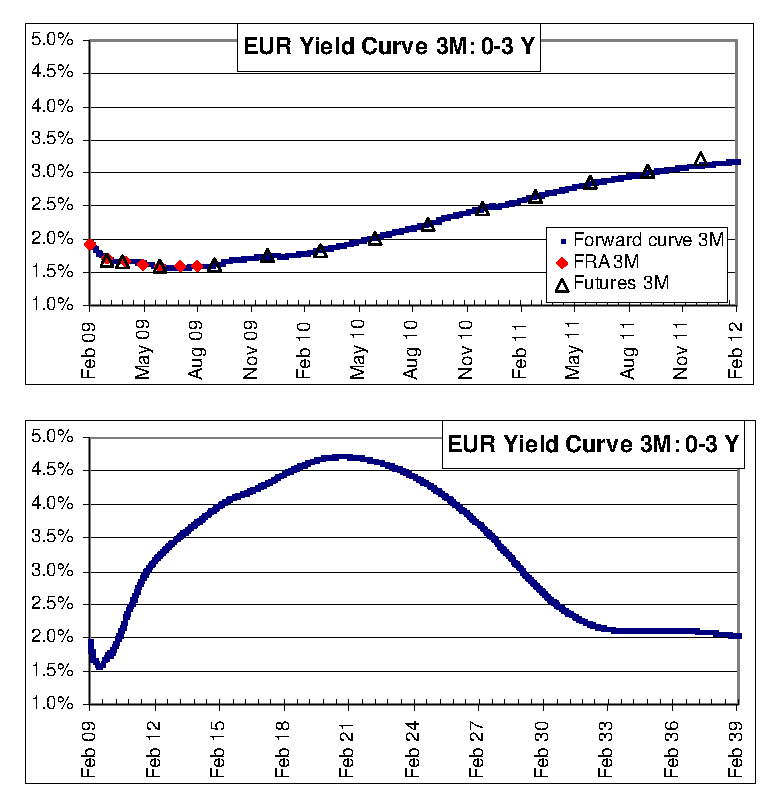
\includegraphics[scale=1.0]{../figures/FigYC3M}
\caption{Forward curve $\mathcal{C}_{3M}^f$ on Euribor3M at 16 Feb. 2009. Plots as in fig. \protect\ref{FigYC1M}. Quoted 3M FRAs and 3M Futures are also reported.}
\label{FigYC3M}
\end{figure}

\begin{figure}[tbp]
\centering
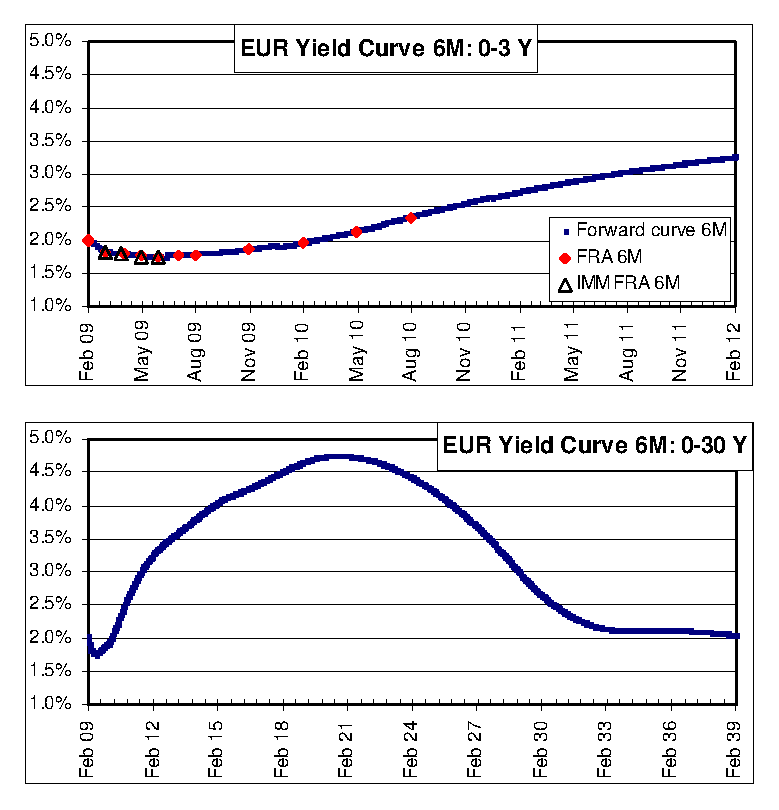
\includegraphics[scale=1.0]{../figures/FigYC6M}
\caption{Forward curve $\mathcal{C}_{6M}^f$ on Euribor6M at 16 Feb. 2009. Plots as in fig. \protect\ref{FigYC1M}. Quoted 6M FRAs and 6M IMM FRAs are also reported.}
\label{FigYC6M}
\end{figure}

\begin{figure}[tbp]
\centering
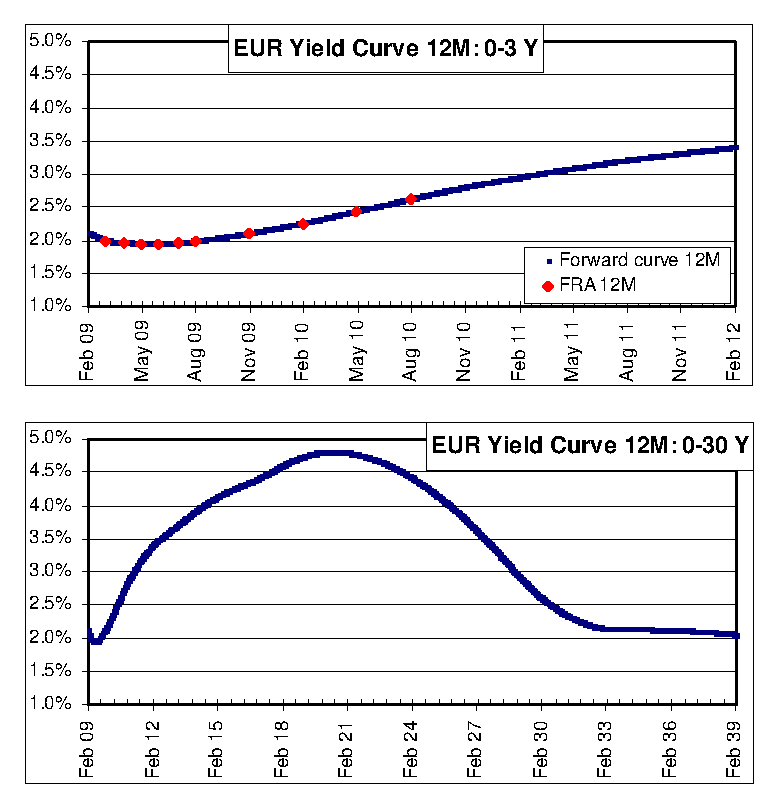
\includegraphics[scale=1.0]{../figures/FigYC12M}
\caption{Forward curve $\mathcal{C}_{12M}^f$ on Euribor12M at 16 Feb. 2009. Plots as in fig. \protect\ref{FigYC1M}. Quoted 12M FRAs are also reported.}
\label{FigYC12M}
\end{figure}


\section{Conclusions}
\label{sec:Conclusions}
We have illustrated a methodology for bootstrapping multiple interest rate yield curves, each homogeneous in the underlying rate tenor, from non-homogeneous plain vanilla instruments quoted on the market.
\par
Results for the concrete EUR market case have been analyzed in detail, showing how real quotations for interest rate instruments on Euribor1M, 3M, 6M and 12M tenor can be used in practice to construct stable, robust and smooth yield curves for pricing and hedging interest rate derivatives.
\par
The full implementation of the work, comprehensive of C++ code and Excel workbooks, is available open source.

\newpage
.
\newpage
.
\newpage
.
\newpage
.
\newpage
%\bibliographystyle{unsrt}
\bibliographystyle{unsrt}
\bibliography{FinanceBibliography}

\end{document}
